\documentclass[sigconf]{acmart}
% Cleaning
\usepackage{pifont}
\usepackage{tikz}
\usepackage{booktabs}
\usepackage{tabularx}
\usepackage{float} % [H]: table right below the heading
\setlength{\textfloatsep}{8pt plus 2pt minus 2pt}
\setlength{\floatsep}{8pt plus 2pt minus 2pt}
\usetikzlibrary{positioning}
\pagestyle{fancy} % removes running headers
\settopmatter{printacmref=false} % Removes citation information below abstract
\renewcommand\footnotetextcopyrightpermission[1]{} % removes footnote with conference information in first column
\pagestyle{plain} % removes running headers
\fancyhead{}
\settopmatter{printacmref=false, printfolios=false}
% Copyright
\setcopyright{none}
\settopmatter{printacmref=false} % Removes citation information below abstract
\acmDOI{}

\setlength{\parskip}{0pt}
\setlength{\parsep}{0pt}
\setlength{\headsep}{0pt}
\setlength{\topskip}{0pt}
\setlength{\topmargin}{0pt}
\setlength{\topsep}{0pt}
\setlength{\partopsep}{0pt}
\linespread{0.95} % Gently compresses lines to help fit 2 pages
\usepackage{mdwlist}
\usepackage{amsmath}

\begin{document}

\title{PluggedIn: Representing Electric Vehicle Charging Accessibility}

\author{Jungwon Youn}
\affiliation{
  \institution{Data Analysis}
  \city{Victoria}
  \state{BC}
  \country{Canada}
}
\email{jungwonyoun@uvic.ca}

\author{Sunghun Cho}
\affiliation{
  \institution{Semantic Modeling}
  \city{Victoria}
  \state{BC}
  \country{Canada}
}
\email{shcho980901@uvic.ca}

\author{Elias Dockal}
\affiliation{
  \institution{Data Modeling}
  \city{Victoria}
  \state{BC}
  \country{Canada}
}
\email{eliasdockal@uvic.ca}


\begin{abstract}
EV charging usability depends on multiple factors, including connector compatibility, operating hours, access conditions, and network information. This project compares existing charging infrastructure data, interoperability protocols, and semantic models to identify differences and gaps in how these factors are represented. Based on this comparison, we design PluggedIn, a data model centered on vehicle-specific practical usability. PluggedIn integrates these factors while explicitly representing adapter compatibility, driver network membership, and structured operating periods, providing a foundation for future knowledge graph representation. The project repository, data models, and related artifacts are available at \url{https://github.com/chohoon901/PluggedIn}
\end{abstract}

% \keywords{Electric Vehicles, Knowledge Graph, Charging Accessibility, Data Modeling, Semantic Interoperability}

\maketitle

% ===============================================================
\section{Introduction}
% ===============================================================
Reliable EV charging requires more than simply locating a charging station. Whether a specific vehicle can use a facility depends on factors such as connector compatibility, operating hours, access restrictions, network and payment conditions, and vehicle-specific suitability~\cite{evkg}.

Existing EV charging information representations model these factors using different structures and for different purposes~\cite{evca}. Therefore, this project investigates and compares how existing EV charging data and models represent and connect such information. Based on the characteristics and differences identified through this comparison, we design the PluggedIn conceptual data model to integrate the information needed to determine the practical usability of charging facilities for specific vehicles.
% ===============================================================
\subsection{History}
% ===============================================================
The representation of energy distribution and refueling infrastructure has evolved alongside changes in information technology. Before computerized data management, information about fueling locations was maintained through analog records such as maps, directories, and administrative documents~\cite{Bauer}. As data management became computerized, such information could be organized in structured digital databases~\cite{nlr}. Web technologies later enabled charging and alternative-fuel infrastructure data to be accessed through online services and APIs, such as the Alternative Fuels Data Center (AFDC)~\cite{afdc_web}.

As EV charging ecosystems became more complex, information beyond facility locations, including connectors, operating conditions, access, and charging actors, became relevant. Different approaches have therefore developed to structure, exchange, and connect this information~\cite{ocpi,oicp,evca}, serving different purposes such as infrastructure data provision, system interoperability, and semantic knowledge representation.

\subsection{Hierarchy of Existing Representations}
Existing EV charging information representations take different forms and structure information according to different purposes and modeling perspectives. We classify the examined representations into three categories: (1) Charging Infrastructure Data Representations, (2) Interoperability Protocols, and (3) Semantic Knowledge Representations.

Charging Infrastructure Data Representations include the National Laboratory of the Rockies (NLR) Alternative Fuels Data Center (AFDC) API, Open Charge Map (OCM), and OpenStreetMap (OSM), which focus on recording and providing real-world charging infrastructure data. NLR and OCM provide structured charging-facility records through APIs~\cite{nlr,ocm}, whereas OSM represents charging facilities as geographic features with tags~\cite{osm}.

Interoperability Protocols, including the Open Charge Point Interface (OCPI) and Open InterCharge Protocol (OICP), standardize information exchange among charging actors and systems. OCPI supports exchange among actors such as CPOs and eMSPs~\cite{ocpi}, while OICP supports eRoaming and related exchange between CPOs and EMPs~\cite{oicp}. Although they also represent charging infrastructure, their primary purpose is interoperability between systems and service providers.

Semantic Knowledge Representations connect EV-related information through semantic concepts and relationships. EVKG connects EVs, charging infrastructure, and connectors through an ontology and knowledge graph~\cite{evkg}, while the Urban EV Charging Activity (EVCA) ontology integrates heterogeneous EV charging data semantically~\cite{evca}. Overall, this classification shows that EV charging information has been modeled for different purposes and from different modeling perspectives.

\begin{figure}[t!]
\centering
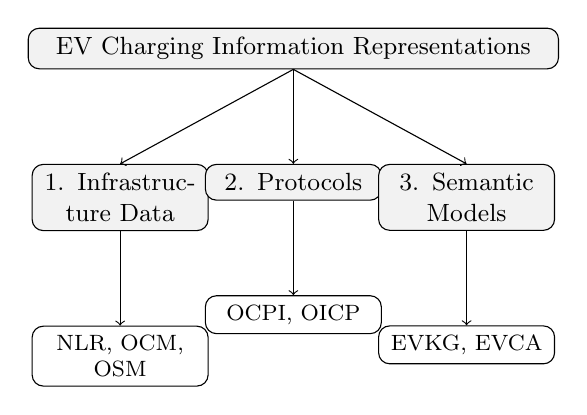
\begin{tikzpicture}[
  node distance=1.2cm and 0.5cm,
  main/.style={rectangle, draw, rounded corners, text width=6.5cm, align=center, fill=gray!10, font=\small},
  sub/.style={rectangle, draw, rounded corners, text width=2.0cm, align=center, fill=white, font=\footnotesize}
]
  \node[main] (root) {EV Charging Information Representations};

  \node[main, below=of root, xshift=-2.2cm, text width=2.0cm] (cat1) {1. Infrastructure Data};
  \node[main, below=of root, xshift=0cm, text width=2.0cm] (cat2) {2. Protocols};
  \node[main, below=of root, xshift=2.2cm, text width=2.0cm] (cat3) {3. Semantic Models};

  \draw[->] (root.south) -- (cat1.north);
  \draw[->] (root.south) -- (cat2.north);
  \draw[->] (root.south) -- (cat3.north);

  \node[sub, below=of cat1, text width=2.0cm] (sub1) {NLR, OCM, OSM};
  \node[sub, below=of cat2, text width=2.0cm] (sub2) {OCPI, OICP};
  \node[sub, below=of cat3, text width=2.0cm] (sub3) {EVKG, EVCA};

  \draw[->] (cat1.south) -- (sub1.north);
  \draw[->] (cat2.south) -- (sub2.north);
  \draw[->] (cat3.south) -- (sub3.north);
\end{tikzpicture}
\caption{Hierarchy of existing EV charging information representations}
\label{fig:hierarchy}
\end{figure}

\section{Comparative Analysis}

The NLR dataset is the official list of alternative-fuel stations operated by the U.S. Department of Energy~\cite{nlr}. It stores each station as a single record, with the network as a string field and operating hours as free text. This makes it difficult to determine whether a station is open at a given time, which account can be used for payment, or whether a port fits the vehicle. Its access restrictions and vehicle-class codes can inform our model.

\begin{table}[!ht]
  \centering
  \caption{Comparison of existing EV charging data models.}
  \label{tab:comparison}
  \scriptsize
  \setlength{\tabcolsep}{3pt}
  \renewcommand{\arraystretch}{1.1}
  \begin{tabularx}{\columnwidth}{@{}l
      >{\raggedright\arraybackslash}X
      >{\raggedright\arraybackslash}X
      >{\raggedright\arraybackslash}X@{}}
    \toprule
    \textbf{Model} & \textbf{Key entities} & \textbf{Strengths} & \textbf{Limitations} \\
    \midrule
    NLR & Station (flat record) & National, open; coded access and vehicle class & Hours as free text; one network field \\
    OCM & POI, Connection, Operator & Per-connector type, power, quantity & Hours in free text; 82\% AFDC-sourced; 19\% missing or unknown operator~\cite{ocm} \\
    OSM & Tagged node or way & Keys for owner, operator, network, hours & Keys rarely filled (owner 0\%)~\cite{osm_data} \\
    OCPI & Location, EVSE, Connector & Structured hours, parking, roles & Not public (B2B only) \\
    EVKG & Station, Network, ConnectorType & Vehicle--connector matching & Hours as string; no adapters or membership \\
    EVCA & Station, Neighbourhood, Trip & Links charging to mobility data & No hours or access; operator only \\
    \bottomrule
  \end{tabularx}
\end{table}
Open Charge Map (OCM) is a crowdsourced charging station platform~\cite{ocm}. It records connector type, power, and quantity separately under each station (POI); about 20\% of BC records have two or more connector types~\cite{ocm}.\footnote{From our analysis of BC extracts retrieved on 5~October~2026: 2,687 OCM stations (OCM API) and 885 OSM stations (Overpass API)~\cite{ocm,osm_data}.} However, operating hours are free text, organizations use a single operator field, and 82\% of BC records identify AFDC as their data provider~\cite{ocm}. Its separation of connectors from stations can inform our model.

OpenStreetMap (OSM) provides keys for owner, operator, network, operating hours, and truck access~\cite{osm}, but they are optional. In our BC extract, the owner key was unused, while network, connector, and operating-hours keys were filled under 22\%~\cite{osm_data}. This illustrates the gap between expressible structure and actual data.

OCPI structures day-of-week operating hours, permitted parking vehicle types, and owner/operator roles within a Location--EVSE--Connector hierarchy~\cite{ocpi}, coming closest to answering our questions. However, its data is exchanged between participating businesses rather than provided as public infrastructure data. Its hierarchy and structured hours can inform our model.

EVKG is a policy-oriented knowledge graph that links electric vehicle adoption, charging infrastructure, and the power grid in the United States~\cite{evkg}. Its direct vehicle--connector compatibility provides a starting point for our model. However, it does not represent adapter-mediated compatibility or driver network membership, and operating hours are represented as strings rather than structured temporal data.

EVCA is an urban-planning ontology linking charging stations, neighbourhoods, and travel data~\cite{evca}. It supports aggregations such as stations per neighbourhood, but does not represent operating hours, access conditions, or vehicle compatibility. Its conversion of OCM data to RDF can guide later stages of our project.


\section{Entity-Relationship Diagram and Project Positioning}
The comparison of existing representations shows that information needed to determine the practical usability of a charging facility is distributed across models with different structures and purposes. PluggedIn therefore centers its conceptual model on whether a specific vehicle can use a charging facility under specific conditions. It integrates vehicle--connector compatibility with operating and access conditions, vehicle suitability, and network information, while addressing several gaps identified in the examined models.

\textbf{Adapter-mediated compatibility.} None of the six models examined represents which adapters are compatible with which connectors. This is relevant as CCS1 and NACS connectors coexist in North America, allowing otherwise incompatible vehicles and chargers to connect through adapters. However, this judgment is often left to the driver; in 21 BC records in our OCM extract~\cite{ocm}, advice to check adapter requirements is provided as free text, while EVKG represents only direct compatibility~\cite{evkg}. PluggedIn therefore introduces an \texttt{Adapter} entity connected to \texttt{ConnectorType} through directional \texttt{ConvertsFrom} and \texttt{ConvertsTo} relationships, with \texttt{MaxPowerKW} representing its power constraint.

\textbf{Network access and membership.} None of the examined models records a driver's network membership. Existing data identifies a station's network, leaving the driver to determine whether it can be used for payment. EVKG, for example, specifies the network directly in the query rather than storing driver memberships~\cite{evkg}. PluggedIn therefore connects \texttt{Driver} to \texttt{Network} through \texttt{MemberOf}, while \texttt{AcceptsGuestPayment} represents whether drivers without network membership can pay at the station.

\textbf{Operating and organizational information.} Several public models store operating hours as free text or mix them with other values, limiting structured queries. PluggedIn therefore separates \texttt{OperatingPeriod} from \texttt{Station}, with \texttt{Day}, \texttt{OpenTime}, and \texttt{CloseTime}. This supports queries for stations with restricted hours, including 77 with explicit numeric schedules in our BC data, of which 21 indicate weekday-only operation and 8 indicate overnight-only operation (5 of which are open 24 hours on weekends)~\cite{ocm}. Organizational information also varies across models. PluggedIn distinguishes \texttt{OwnedBy}, \texttt{OperatedBy}, and \texttt{ServedBy}, and uses an ISA structure for \texttt{Organization}, allowing an organization to be stored once while playing multiple roles.

Since the final goal is a knowledge graph, the ERD was designed with semantic representation in mind. \texttt{ConnectorType} is modeled as an entity so that differently named connectors across sources can share one \texttt{ConnectorType}, while relationships are named as verbs that can later serve as triple predicates. Relationships with attributes, such as \texttt{MemberOf}, can later be represented through a separate \texttt{Membership} node.

\bibliographystyle{ACM-Reference-Format}
\bibliography{bibliography.bib}
\begin{figure*}[p]
  \centering
  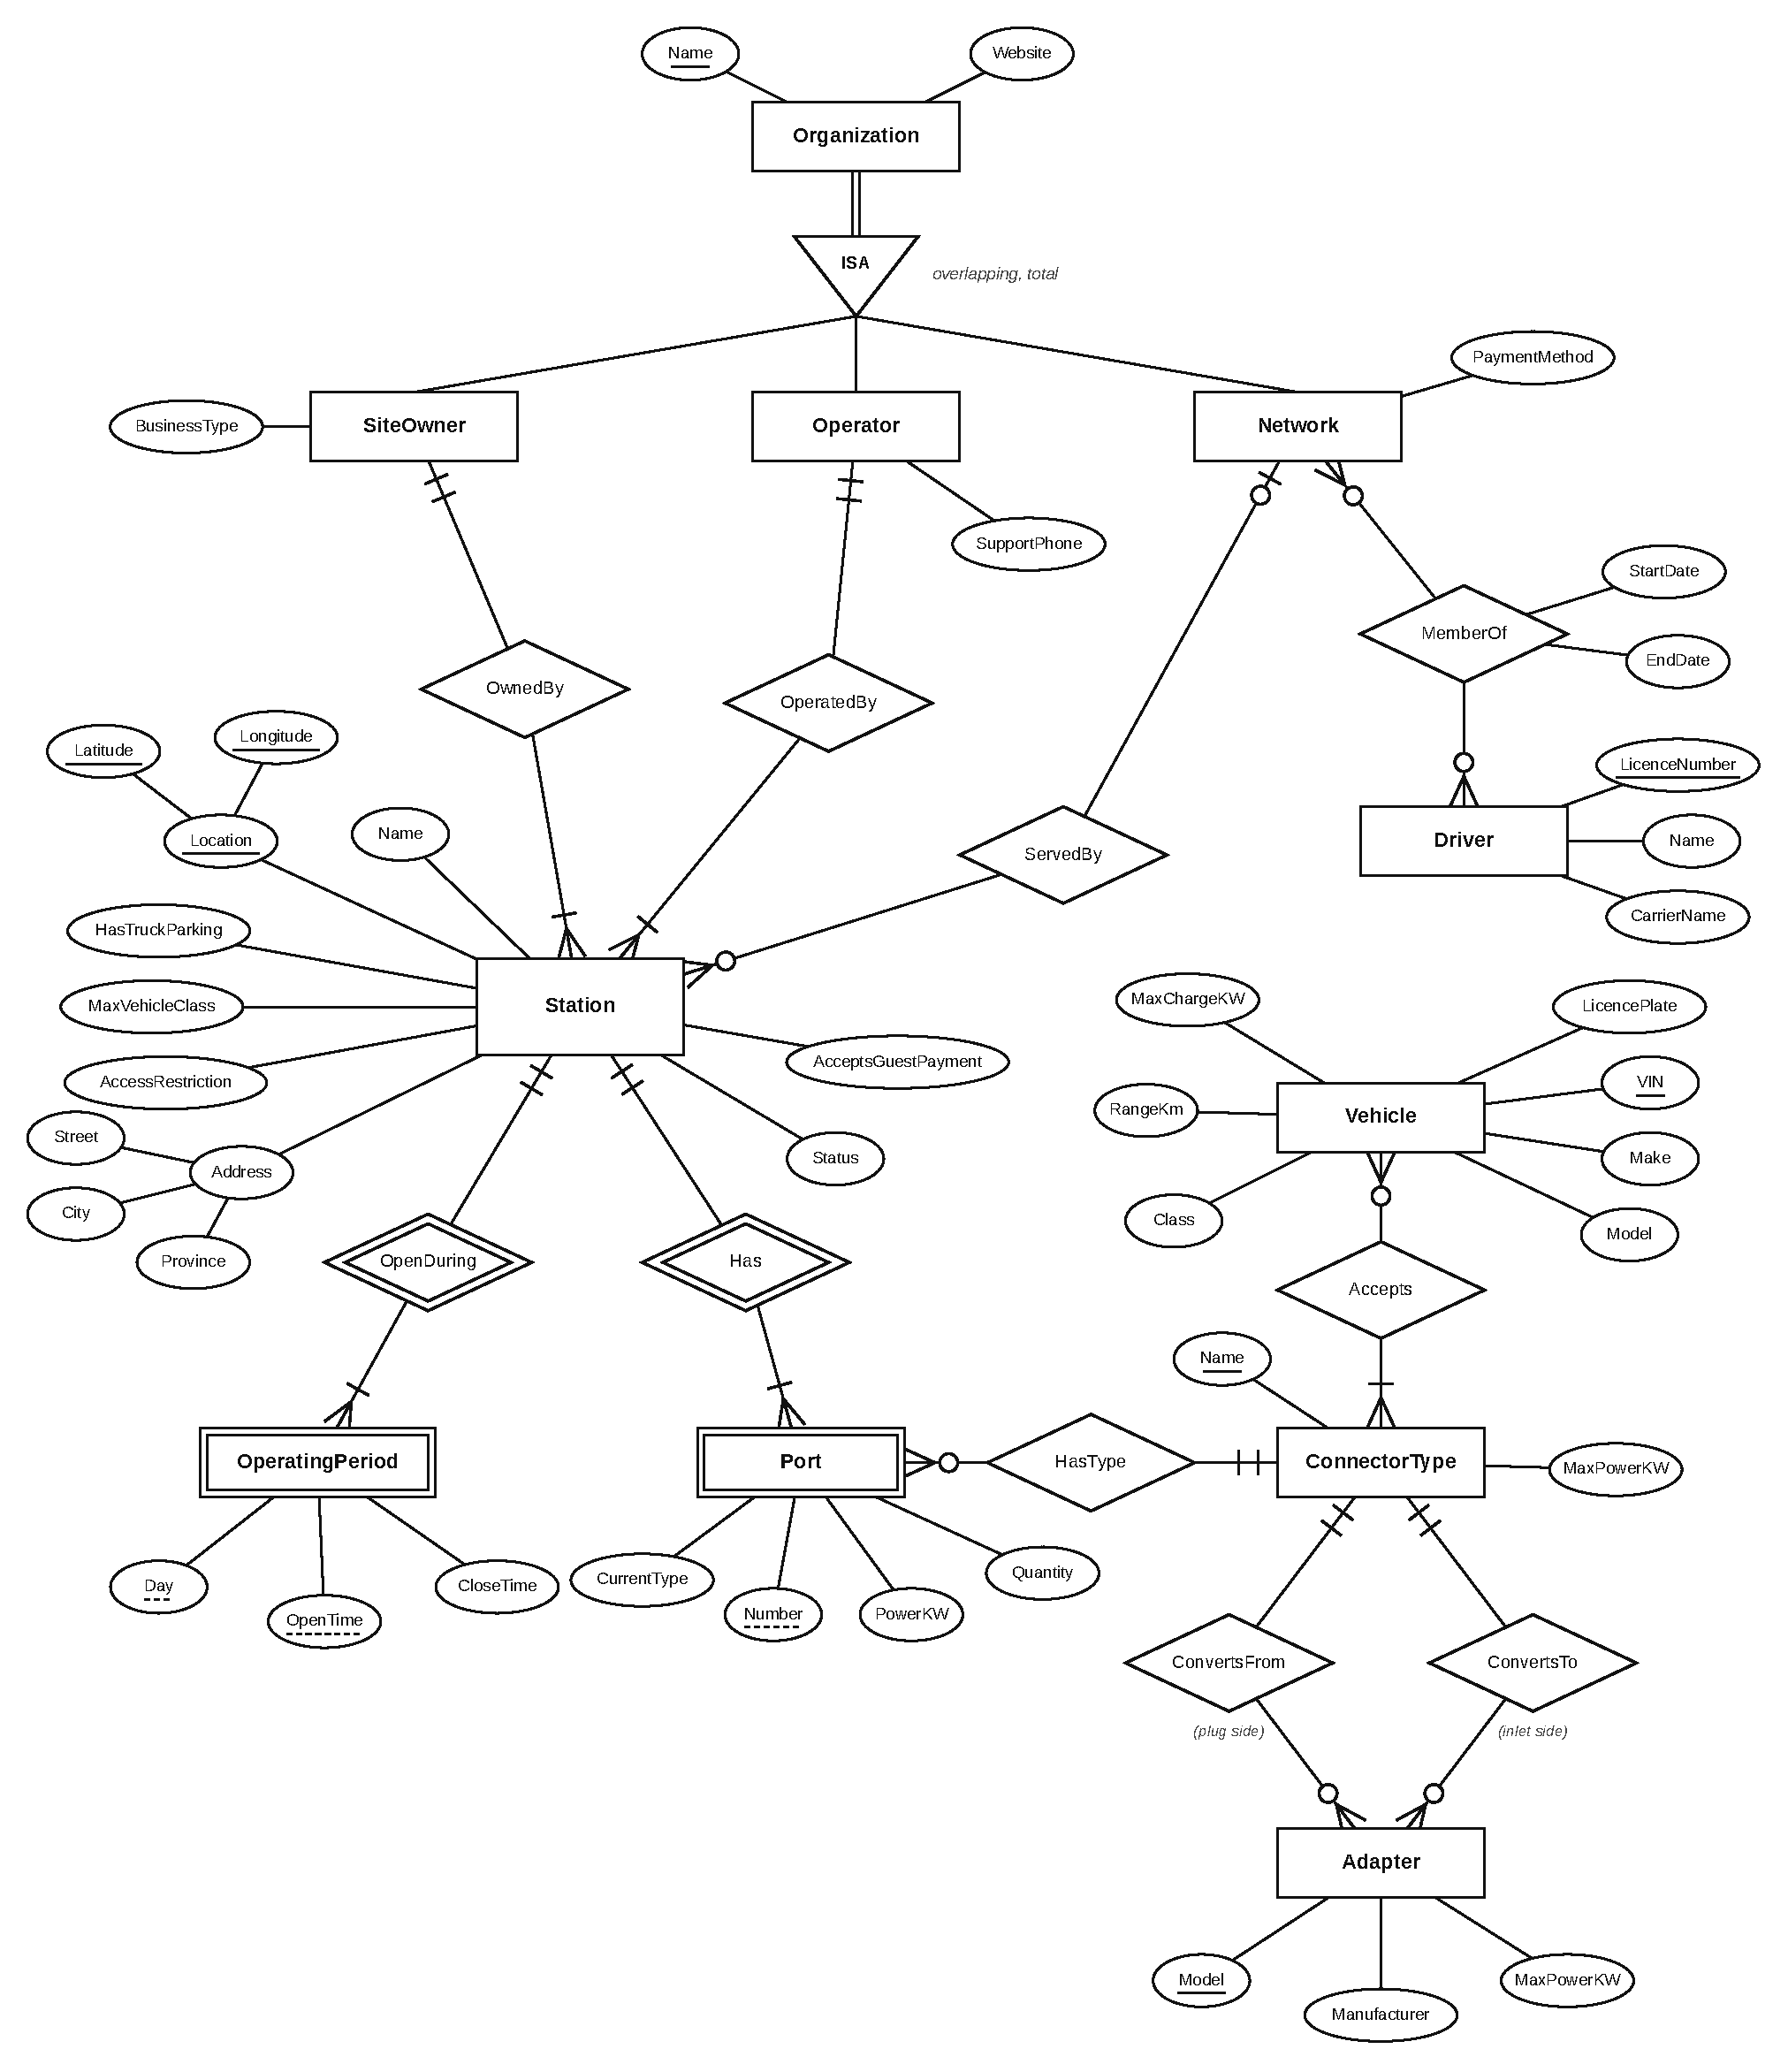
\includegraphics[width=\textwidth]{pluggedin_erd_portrait.pdf}
  \caption{The draft version of our project's ER diagram.}
  \label{fig:erd}
\end{figure*}



\clearpage
\appendix
\section{Appendix: Original Draft Before AI-Assisted Editing}
\subsection{Abstract}

EV charging usability depends on multiple factors, including connector compatibility, operating hours, access conditions, and network information. This project compares existing charging infrastructure data, interoperability protocols, and semantic models to identify differences and gaps in how these factors are represented. Based on this comparison, we design PluggedIn, a data model centered on vehicle-specific practical usability. PluggedIn integrates these factors while explicitly representing adapter compatibility, driver network membership, and structured operating periods, providing a foundation for future knowledge graph representation. The project repository, data models, and related artifacts are available at https://github.com/chohoon901/PluggedIn


\subsection{Introduction}

Reliable EV charging requires more than simply locating a charging station. Whether a specific vehicle can use a facility depends on factors such as connector compatibility, operating hours, access restrictions, network and payment conditions, and vehicle-specific suitability.

Existing EV charging information representations model these factors using different structures and for different purposes. Therefore, this project investigates and compares how existing EV charging data and models represent and connect such information. Based on the characteristics and differences identified through this comparison, we design the PluggedIn conceptual data model to integrate the information needed to determine the practical usability of charging facilities for specific vehicles.


\subsection{History}

How we track fuel and energy infrastructure has changed a lot with transportation over time. Long before computer networks, finding fuel meant using analog things like paper maps, travel directories, and local books. Back then, travelers had to manually check separate, static records just to find a place to stop.

Later, as computers got better, data moved into relational databases. Public and private groups started putting station coordinates and grid info into digital tables, but these databases usually stayed locked inside separate company systems. When the internet and web apps came along, APIs—like the Alternative Fuels Data Center (AFDC)—finally made station data available online.

Still, because these platforms were built separately, they ended up with messy schemas, different naming styles, and lots of free text. This is why we are moving toward semantic web tech and knowledge graphs today: they help connect vehicle specs, connector types, and access rules into one machine-readable system.

\subsection{Hierarchy of Existing Representations}

Existing systems for representing EV charging information do not exist in a single form; they consist of various forms such as data, protocols, and knowledge graphs. Although these representations address the same EV charging domain, they structure the information differently depending on their primary purpose and modeling perspective. In this project, the investigated existing representations were classified into three categories based on these differences: (1) representation of charging infrastructure, (2) information exchange and interoperability protocols, and (3) meaning-based knowledge representation.

The first category, Charging Infrastructure Data Representations, includes the NLR AFDC API, OCM, and OSM. They focus on recording and providing data related to real-world charging facilities and their information. The NLR AFDC API provides structured information on alternative fuel and EV charging stations in the United States, while OCM offers publicly collected data such as charging POIs, connections, operators, and usage in the form of a database and APIs. OSM represents charging facilities as geographic features in the real world and uses tags to indicate their associated attributes. While they all share the commonality of representing charging infrastructure as data, the modeling approaches differ in that NLR and OCM provide charging facility information as structured records, whereas OSM uses geographic objects and tags.

The second category, Interoperability Protocols, includes OCPI and OICP. Their primary goal is not merely to store and provide charging information, but to standardize and exchange information among different charging actors and systems. OCPI is a protocol for exchanging charging information between entities such as CPOs and eMSPs, while OICP supports eRoaming and related information exchange between CPOs and EMPs. Both protocols also describe charging infrastructure in detail, but unlike NLR, OCM, and OSM, their primary purpose is to support information exchange and interoperability among different systems and operators.

The third category, Semantic Knowledge Representations, includes EVKG and EVCA. They focus not merely on storing or exchanging information related to EV charging, but on explicitly expressing and linking the meanings of different concepts and relationships. EVKG connects various concepts such as EVs, charging infrastructure, and connectors through ontology and knowledge graphs, while EVCA focuses on meaningfully integrating previously isolated EV charging-related data silos based on ontology. Although the two models differ in specific scope and approach, they share the common feature of providing machine-interpretable and interoperable representations by linking EV charging information through semantic relationships. These classifications show that EV charging information has been modeled according to different purposes and perspectives: representing actual infrastructure data, facilitating information exchange between systems, and expressing meaning-based knowledge.

\subsection{Comparative analysis}

The NLR dataset is the official list of alternative-fuel charging and fuelling stations operated by the U.S. Department of Energy. It stores each station as a single record, with the network as a single string field and operating hours as free text. As a result, access restrictions and vehicle class can be determined from codes, but it is difficult to determine whether a station is open at a given time, which account can be used for payment, or whether a port fits the vehicle. It is the origin of Canadian charging station data, and its approach of encoding access restrictions and vehicle class as codes can be a reference for our project.

Open Charge Map (OCM) is a crowdsourced charging station platform. This dataset records the type, power, and quantity of each connector separately under each station (POI), which shows that about 20\% of BC stations have two or more connector types. However, operating hours are mixed into free text, organizations are represented by a single operator field, and 83\% of BC records come from the U.S. Department of Energy dataset, so they inherit its limitations. Its structure of separating connectors from stations is a direct reference for our project.

OpenStreetMap (OSM) provides keys for owner, operator, network, operating hours, and truck access in its schema, but none of these keys is enforced; among 885 stations in BC, the owner key was never used, and the network, connector, and operating-hours keys were filled for 22\% or less. In other words, it shows the gap between the structure that can be expressed and the data that is actually expressed.

OCPI is a roaming protocol between businesses that structures day-of-week operating hours, permitted parking vehicle types, and owners and operators within a location–EVSE–connector hierarchy, and among the compared models it comes closest to answering our questions. However, this data is exchanged only between contracted businesses and is not public, so the necessary structure exists in industry but not in public data. Its three-level hierarchy and day-of-week operating-hours structure can be a reference for our project.

EVKG is a policy-oriented knowledge graph that links electric vehicle adoption, charging infrastructure, and the power grid in the United States. By representing direct vehicle–connector compatibility, it serves as the starting point for our model. However, it does not represent adapter-mediated compatibility or a driver's network membership, and its operating hours are strings and therefore not machine-readable.

EVCA is an urban-planning ontology that links charging station, neighbourhood, and travel data in Eindhoven. It is designed for aggregations such as the number of charging stations per neighbourhood or per operator. Because it has no operating hours, access conditions, or vehicle compatibility, it cannot answer whether an individual station can be used now. Its process of converting OCM data into RDF can be a reference for later stages of our project.


\subsection{Entity-Relationship Diagram And Project Positioning}

Public models have a weak structure, industry standards are not public, and adapter compatibility and driver membership are not found anywhere. Therefore, the key strength of our ERD is that it is open source and multi-source, combining the strengths of the existing models.

First, none of the six models above shows which adapter is compatible with which connector. To solve this problem, we made an Adapter entity and connected it to the ConnectorType entity, so that it can be linked to Port and Vehicle. Because of this, after converting it into a knowledge graph, we can answer the question "Can this vehicle charge at a port of this charging station?" in an extended way. Second, whether a driver has joined a certain network also could not be found in the models above. By connecting the Driver entity and the Organization.Network entity, we made it possible to answer the question "Can I pay at that charging station?". Besides these, we can find other gaps of our own project, and free-text operating hours is one of them. Most of the models above store operating hours as free text, and sometimes values that are not operating hours are mixed in, so a machine cannot read them. For this, we separated the OperatingHour entity from the Station entity, and because of this, not only the case where a station is open 24 hours but also the case where it is open only at certain times, where a driver is more likely to make a wasted trip, can be used in queries. The Port entity is also a similar text parsing case. We checked that in the NLR dataset, ports were attached to the Station entity. This can cause a data duplication problem, because in the existing dataset we found that more than 20\% of Ports have two or more values. As a similar problem, in most models the owner, operator, and network of a charging station were grouped as an array in one field, or only one field was used. To solve this, we also applied an ISA structure to the Organization entity and separated it into owner, operator, and network, so that we prevent the case where many values are stored with duplication in one entity, and the case where many values are stored in one field as free text or a list.

Since the final goal of this project is not to finish with just making an ERD but to make a knowledge graph, we kept thinking about how the knowledge graph should be made while designing the ERD as well. We made ConnectorType an entity so that we can check whether connectors with different names from different sources are the same, and we named relationships as verbs so that they are easy to use as the verbs of triples. For relationships that have attributes like MemberOf, we plan to put Membership as a separate node to express those attributes.

\end{document}
